%%%%%%%% Klassen-Optionen
\documentclass[12pt,a4paper]{scrartcl}

%%%%%%%% PAKETE: unverzichtbare Pakete mit Einstellungen
\usepackage[left=2.5cm, right=2cm, top=3cm, bottom=3cm, a4paper]{geometry} %Seitenrände
\usepackage[utf8x]{inputenc} % utf8-Kodierung und direkte Eingabe von Sonderzeichen
\usepackage{fixltx2e} % Verbessert einige Kernkompetenzen von LaTeX2e

%%%%%%%% PAKETE: AMS-Pakete
\usepackage{amsmath} % Mathe-Erweiterung
\usepackage{amsfonts} % Schrift-Erweiterung
\usepackage{amssymb} % Sonderzeichen-Erweiterung

%%%%%%%% PAKETE: Sonstiges
\usepackage[colorlinks, citecolor=black, filecolor=black, linkcolor=black, urlcolor=black]{hyperref} % Links
\usepackage{wrapfig} % ausgeklügekte Floatumgebung
\usepackage{float} % normale Floatumgebung
\restylefloat{figure} % ermöglicht die Verwendung von "H" (ist noch stärker als "h!")
\usepackage[small,it,singlelinecheck=false]{caption} % Bildunterschriften formatieren
\usepackage{multirow} % ermöglich Verbinden von Tabellenzeilen
\usepackage{multicol} % ermöglicht Spalten
\usepackage{fancyhdr} % ermöglicht Kopf- und Fußzeilen
\usepackage{graphicx} % Einbinden von Bildern möglich
\usepackage{units} % Einheiten
\usepackage{subcaption}

%%%%%%%% DEFINITIONEN: Titelseite
\author{April Cooper, Patrick Kreissl und Sebastian Weber}
\title{Worksheet 5:  Monte-Carlo}
\publishers{University of Stuttgart}
\date{\today}

%%%%%%%% ANPASSUNGEN: Kopf-und Fußzeile
\fancypagestyle{plain}{} % redefine the plain pagestyle to match the fancy layout
\pagestyle{fancy} % aktiviere eigenen Seitenstil
\fancyhf{} % alle Kopf- und Fußzeilen bereinigen
\fancyhead[L]{Worksheet 5:  Monte-Carlo}
\fancyhead[R]{\today}
\renewcommand{\headrulewidth}{0.6pt} % obere Trennlinie
\fancyfoot[L]{April Cooper, Patrick Kreissl und Sebastian Weber}
\fancyfoot[R]{Page \thepage}
\renewcommand{\footrulewidth}{0.6pt} % untere Trennlinie

%%%%%%%% ANPASSUNGEN: Absätze
\setlength{\parindent}{0em} % keine Absatzeinzüge
\setlength{\parskip}{0em} % Absatz-Abstand

%%%%%%%% ANPASSUNGEN: Abbildungsverzeichnis
\usepackage{tocloft} % Zum Anpassen der Verzeichnisse
\renewcommand{\cftfigpresnum}{Abb. }
\renewcommand{\cfttabpresnum}{Tab. }
\renewcommand{\cftfigaftersnum}{:}
\renewcommand{\cfttabaftersnum}{:}
\setlength{\cftfignumwidth}{2cm}
\setlength{\cfttabnumwidth}{2cm}
\setlength{\cftfigindent}{0cm}
\setlength{\cfttabindent}{0cm}

%%%%%%%% SONSTIGES
\usepackage{pdfpages}
\usepackage{pgf}

% NÜTZLICH: http://truben.no/latex/table/

% Anfang des eigentlichen Dokuments
\begin{document}

\maketitle
\tableofcontents
\newpage

% =============== Section ============
\section{Simple Sampling- Intrgration}
First we were asked to program a function runge(x) that computes the runge function\newline \(f(x) = \frac{1}{1+x^2}\) and to plot it on the interval $[-5,5]$.
\begin{figure}[H]
\centering
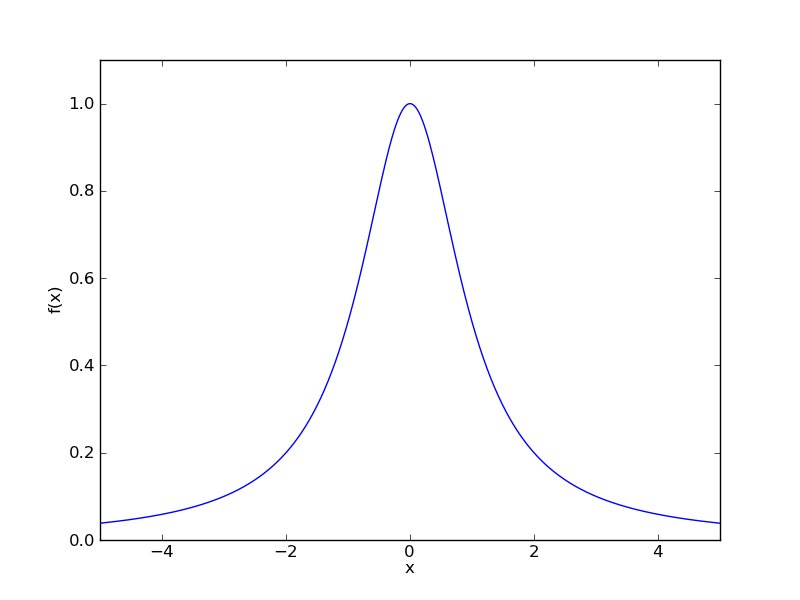
\includegraphics[width=16.0cm]{../plots/runge.png}
\caption{Runge function f(x) on the interval [-5,5]}
\label{fig:runge}
\end{figure}
Then we had to write a function that computes the exact integral of the runge function.
The exact result is: \[\int^{5}_{-5}\frac{1}{1+x^2} =  arctan(5)-arctan(-5) \approx 2.7468 \]

After that we were asked to program a function simple\_sampling(f,a,b,N) that performs N steps of a simple sampling Monte-Carlo integration and to use this function to compute the Integral for $N=2^{i}$ with $2\le i\le 20$.
Furthermore we were asked to determine the actual and statistical error and to plot them against the number of integration steps N.
In the following are two plots of the error from two different  runs. 
 
 \begin{figure}[H]
\centering
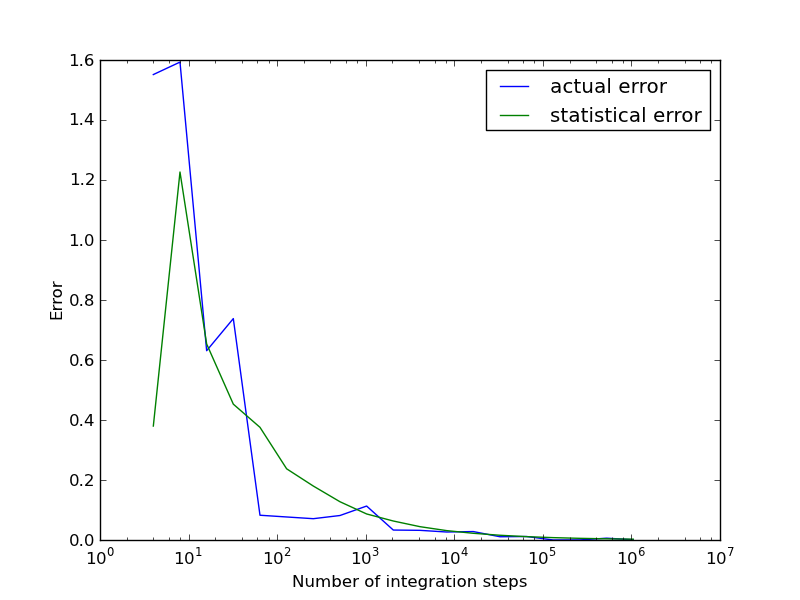
\includegraphics[width=16.0cm]{../plots/Error2.png}

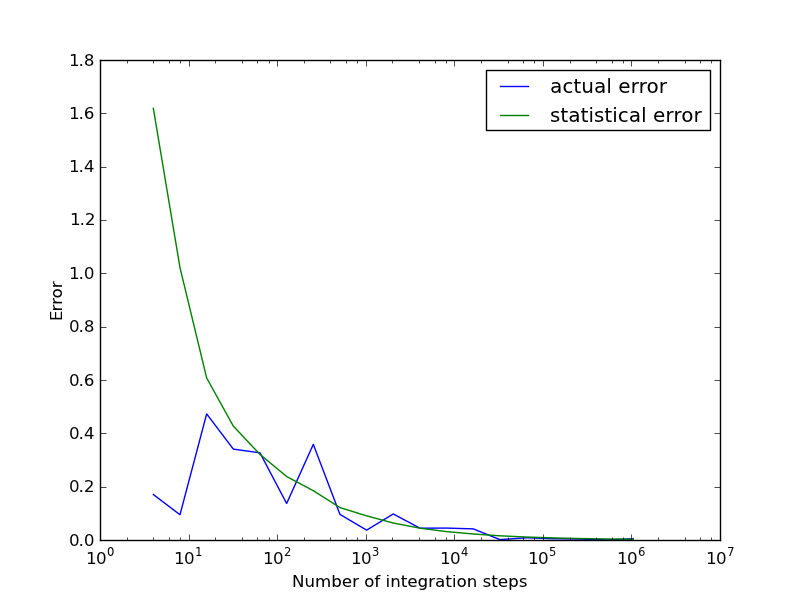
\includegraphics[width=16.0cm]{../plots/Error3.png}
\caption{Statistical and actual error of the Integration with the simple sampling method}
\label{fig:error1}
\end{figure}

As it can be seen due to the randomness of the points in which f is evaluated the actual error behaves quite different from run to tun. Furthermore it also varies for small numbers of integration steps quite a lot from the statistical error. In contrast to this the statistical error has a much more comparable behavior in different runs.

\section{Importance Sampling- Metropolis-Hastings-Algorithm}
In this task we were asked to implement the Metropolis-Hastings-algorithm and to use that function to generate a given number of samples for several $\Delta x$ being used in the trial move.
The resulting histograms can be found in the following plots
 \begin{figure}[H]
\centering
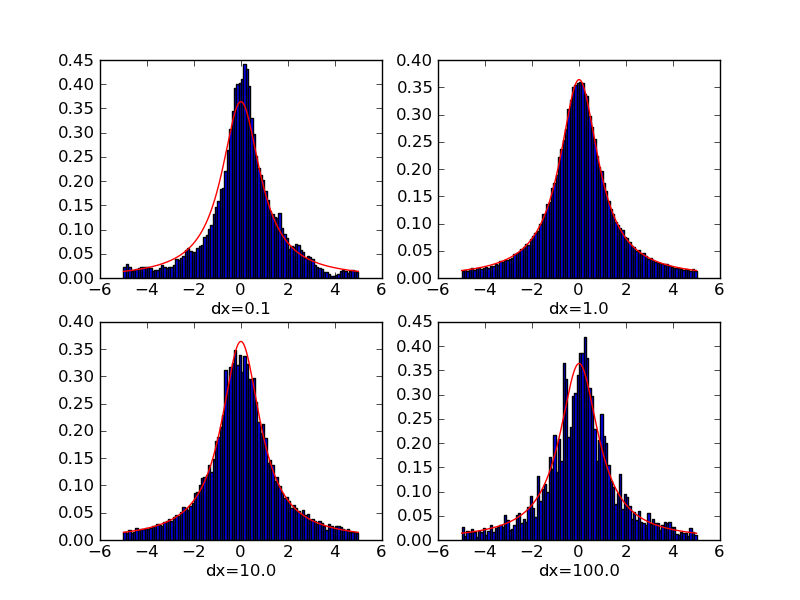
\includegraphics[width=16.0cm]{../plots/hist.png}
\caption{Distribution histograms of the Metropolis samples with 100 bins compared to the normalized runge function (red)}
\label{fig:runge}
\end{figure}
By eye it is hard to say wether $dx = 1.0$ or $dx= 1.0$ is the better choice. Having a look at the acceptance rates - $\approx 84.8\%$ for $ dx=1.0$, $\approx 32.5\%$ for $dx=10.0$  -and taking into account that it was stated on the worksheet that an acceptance rate of about $30\%$ is optimal, it can be said that $dx = 10.0 $ is a better choice than $dx= 1.0$.


\end{document}


% =============== Comments ============
\begin{comment}
\verb{x_init {}}

\begin{figure}[H]
	\resizebox{1\textwidth}{!{\input{../plots/NAME.pgf}}
	\caption{CAPTION}\label{fig:NAME}
\end{figure}
\end{comment}
